%%%%%%%%%%%%%%%%%%%%%%%%%%%%%%%%%%%%%%%%%%%%%%%%
% E.Pinault-Bigeard - s2i@pinault-bigeard.com
% http://s2i.pinault-bigeard.com
% CC BY-NC-SA 2.0 FR - http://creativecommons.org/licenses/by-nc-sa/2.0/fr/
%%%%%%%%%%%%%%%%%%%%%%%%%%%%%%%%%%%%%%%%%%%%%%%%
\documentclass[11pt]{article}

%%%%%%%%%%%%%%%%%%%%%%%%%%%%%%%%%%%%%%%%%%%%%%%%
% Package UPSTI_Document
%%%%%%%%%%%%%%%%%%%%%%%%%%%%%%%%%%%%%%%%%%%%%%%% 
\RequirePackage{UPSTI_Document}
\usepackage{stmaryrd}
\usetikzlibrary{snakes}

%---------------------------------%
% Paramètres du package
%---------------------------------%

% Version du document (pour la compilation)
% 1: Document prof
% 2: Document élève
% 3: Document à publier
\newcommand{\UPSTIidVersionDocument}{2}

% Choix du type de document
% 10: Mémo
\newcommand{\UPSTIidTypeDocument}{10}

% Thiers
\newcommand{\UPSTIvariante}{2}

% Classe
% 2: PT
\newcommand{\UPSTIidClasse}{2}

% Titre
\newcommand{\UPSTItitreEnTete}{Outils mathématiques}      

% Source
\newcommand{\UPSTImessage}{Rappels de PTSI}

% Source
%\newcommand{\UPSTIsource}{E.PINAULT-BIGEARD}

% Versioning
\newcommand{\UPSTInumeroVersion}{1.1}
                 
%----------------------------------------------- 
\UPSTIcompileVars		% "Compile" les variables
%%%%%%%%%%%%%%%%%%%%%%%%%%%%%%%%%%%%%%%%%%%%%%%% 


%%%%%%%%%%%%%%%%%%%%%%%%%%%%%%%%%%%%%%%%%%%%%%%% 
% Début du document
%%%%%%%%%%%%%%%%%%%%%%%%%%%%%%%%%%%%%%%%%%%%%%%% 
\begin{document}

% Création de l'en-tête
\UPSTIbuildPage 
\section{Trigonométrie}
\subsection{Cercle trigonométrique}
Une lecture efficace du cercle trigonométrique permet de rapidement les relations suivantes:

	\begin{center}	
    \begin{tikzpicture}[scale=3.6]
		        % Cercle et axes
        \draw[gray] (-1,0) -- (1,0);
        \draw[gray] (0,-1) -- (0,1);
        \draw[thick] (0,0) circle(1);

		% 3 angles principaux
        \foreach \x in {30,45,60} {
                \draw[gray, dashed] (0,0) -- (\x:1);
                % dots at each point
                \filldraw[black] (\x:1) circle(0.4pt);
        }

%      \foreach \x in {0,30,...,360} {
%                % lines from center to point
%                \draw[gray] (0cm,0cm) -- (\x:1cm);
%                % dots at each point
%                \filldraw[black] (\x:1cm) circle(0.4pt);
%                % draw each angle in degrees
%                \draw (\x:0.6cm) node[fill=white] {$\x^\circ$};
%        }
%
%        % draw each angle in radians
%        \foreach \x/\xtext in {
%            30/\frac{\pi}{6},
%            45/\frac{\pi}{4},
%            60/\frac{\pi}{3},
%            90/\frac{\pi}{2},
%            120/\frac{2\pi}{3},
%            135/\frac{3\pi}{4},
%            150/\frac{5\pi}{6},
%            180/\pi,
%            210/\frac{7\pi}{6},
%            225/\frac{5\pi}{4},
%            240/\frac{4\pi}{3},
%            270/\frac{3\pi}{2},
%            300/\frac{5\pi}{3},
%            315/\frac{7\pi}{4},
%            330/\frac{11\pi}{6},
%            360/2\pi}
%                \draw (\x:0.85cm) node[fill=white] {$\xtext$};
%
%        \foreach \x/\xtext/\y in {
%            % the coordinates for the first quadrant
%            30/\frac{\sqrt{3}}{2}/\frac{1}{2},
%            45/\frac{\sqrt{2}}{2}/\frac{\sqrt{2}}{2},
%            60/\frac{1}{2}/\frac{\sqrt{3}}{2},
%            % the coordinates for the second quadrant
%            150/-\frac{\sqrt{3}}{2}/\frac{1}{2},
%            135/-\frac{\sqrt{2}}{2}/\frac{\sqrt{2}}{2},
%            120/-\frac{1}{2}/\frac{\sqrt{3}}{2},
%            % the coordinates for the third quadrant
%            210/-\frac{\sqrt{3}}{2}/-\frac{1}{2},
%            225/-\frac{\sqrt{2}}{2}/-\frac{\sqrt{2}}{2},
%            240/-\frac{1}{2}/-\frac{\sqrt{3}}{2},
%            % the coordinates for the fourth quadrant
%            330/\frac{\sqrt{3}}{2}/-\frac{1}{2},
%            315/\frac{\sqrt{2}}{2}/-\frac{\sqrt{2}}{2},
%            300/\frac{1}{2}/-\frac{\sqrt{3}}{2}}
%                \draw (\x:1.25cm) node[fill=white] {$\left(\xtext,\y\right)$};
                
                
		% cos
        \foreach \x/\xtext in {
            0.5/\frac{1}{2},
            0.707/\frac{\sqrt{2}}{2},
            0.866/\frac{\sqrt{3}}{2}}
                \draw[gray] (\x,0.03) -- (\x,-0.03) node[below,gray] {$\xtext$};

		% sin
        \foreach \x/\xtext in {
            0.5/\frac{1}{2},
            0.707/\frac{\sqrt{2}}{2},
            0.866/\frac{\sqrt{3}}{2}}
                \draw[gray] (0.03,\x) -- (-0.03,\x) node[left,gray] {$\xtext$};
		
        % draw each angle in radians
        \foreach \x/\xtext in {
            30/\frac{\pi}{6},
            45/\frac{\pi}{4},
            60/\frac{\pi}{3}}
                \draw (\x:1.1cm) node[gray] {$\xtext$};


		\draw[dashed,UPSTIcustomColor1] (15:1) rectangle (195:1);
		\draw[dashed,UPSTIcustomColor1] (75:1) rectangle (255:1);
        \foreach \x in {15,75,105,165,195,255,285,345} {
                \filldraw[UPSTIcustomColor1] (\x:1) circle(0.4pt);
        }
        \foreach \x/\xtext in {
            15/\theta,
            75/\frac{\pi}{2}-\theta,
            105/\frac{\pi}{2}+\theta,
            165/\pi-\theta\quad,
            195/\pi+\theta\quad,
            255/-\frac{\pi}{2}-\theta,
            285/-\frac{\pi}{2}+\theta,
            345/-\theta}
                \draw (\x:1.1cm) node[UPSTIcustomColor1] {$\xtext$};


		\node[align=left] at (-1.05,1.2) {
			$\displaystyle\cos\left(\frac{\pi}{2}+\theta\right)=-\sin\theta$\\
			\\
			$\displaystyle\sin\left(\frac{\pi}{2}+\theta\right)=\cos\theta$
		};
		\node[align=left] at (1.15,1.2) {
			$\displaystyle\cos\left(\frac{\pi}{2}-\theta\right)=\sin\theta$\\
			\\
			$\displaystyle\sin\left(\frac{\pi}{2}-\theta\right)=\cos\theta$
		};

		\node[align=left] at (-1.6,0.5) {
			$\displaystyle\cos\left(\pi-\theta\right)=-\cos\theta$\\
			$\displaystyle\sin\left(\pi-\theta\right)=\sin\theta$
		};

		\node[align=left] at (-1.6,-0.5) {
			$\displaystyle\cos\left(\pi+\theta\right)=-\cos\theta$\\
			$\displaystyle\sin\left(\pi+\theta\right)=-\sin\theta$
		};

		\node[align=left] at (1.55,-0.5) {
			$\displaystyle\cos\left(-\theta\right)=\cos\theta$\\
			$\displaystyle\sin\left(-\theta\right)=-\sin\theta$
		};
    \end{tikzpicture}
\end{center}	


\subsection{Relations entre cos, sin et tan}
\vspace{-1em}
\noindent
\begin{minipage}[c]{0.45\linewidth}
\[ \cos^2\theta + \sin^2\theta=1\] 
\end{minipage} \hfill
\begin{minipage}[c]{.45\linewidth}
\[1+\tan^2\theta=\dfrac{1}{\cos^2\theta} \]
\end{minipage} 


\subsection{Formules d'addition}
\vspace{-1em}
\noindent
\begin{minipage}[c]{0.45\linewidth}
\[ \cos(a-b)=\cos a\cos b+\sin a\sin b\]
\[ \sin(a-b)=\sin a\cos b-\cos a\sin b\]
\[ \tan(a-b)=\dfrac{\tan a-\tan b}{1+\tan a\tan b} \]
\end{minipage} \hfill
\begin{minipage}[c]{.45\linewidth}
\[ \cos(a+b)=\cos a\cos b-\sin a\sin b\] 
\[ \sin(a+b)=\sin a\cos b+\cos a\sin b\] 
\[ \tan(a+b)=\dfrac{\tan a+\tan b}{1-\tan a\tan b} \]
\end{minipage} 


\subsection{Formules de linéarisation}
\vspace{-1em}
\noindent
\begin{minipage}[c]{0.3\linewidth}
\[ \cos^2\theta =\dfrac{1+\cos(2\theta)}{2}\] 
\end{minipage} \hfill
\begin{minipage}[c]{.3\linewidth}
\[ \sin^2\theta =\dfrac{1-\cos(2\theta)}{2}\] 
\end{minipage} \hfill
\begin{minipage}[c]{.3\linewidth}
\[ \tan^2\theta =\dfrac{1-\cos(2\theta)}{1+\cos(2\theta)}\] 
\end{minipage} 


\section{Calcul vectoriel}
Les théories de la mécanique utilisent des grandeurs qui peuvent mathématiquement être représentées par des vecteurs (vitesse, position, accélération, force...). Ces vecteurs sont des éléments d'espaces vectoriels euclidiens sur $\mathbb{R}$ de dimension 3 noté $(E)$. Les grandeurs vecteurs sont intrinsèques, elles sont indépendantes de la base dans laquelle elles sont représentées. 

\subsection{Définitions}

Soient deux points $A$ et $B$. $(A,B)$ est appelé un bipoint. Un bipoint est défini par son origine $A$, son sens (de $A$ vers $B$), sa direction (droite $(AB)$) et sa norme (distance de $A$ à $B$). 

Un vecteur   est l'ensemble des bipoints équipollents (parallèles, même sens, même norme) au bipoint $(A,B)$.

\begin{wrapfigure}{r}{8cm}
  \centering
  \vspace{-2em}
\begin{tikzpicture}
\node[inner sep = 0] (a) at (0,0) {} node[above left,xshift=-2mm] {$A$} ;
\draw (a)-- ++(200:0.5);
\draw[very thick,->,>=latex,UPSTIcustomColor1] (a) -- ++(20:3) node[midway,above left,black] {$\vv V$} node[above right,yshift=2mm,black] {$B$} node[inner sep=0] (b) {};
\draw (b) -- ++(20:1) node[right] {(D)};
\draw (a) -- ++ (110:1) node[inner sep=0] (a1){};
\draw (b) -- ++ (110:1) node[inner sep=0] (b1){};
\draw[<->,>= latex] (a1) -- (b1) node[above,midway,sloped] {Norme};
\draw[very thick,->,>=latex,UPSTIcustomColor1] (2,-0.5) -- ++(20:3) node[midway,above left,black] {$\vv V$};
\draw[very thick,->,>=latex,UPSTIcustomColor1] (3.5,-1) -- ++(20:3) node[midway,above left,black] {$\vv V$};
\end{tikzpicture}
  \vspace{-2em}
\end{wrapfigure}

\noindent Pour le vecteur, on définit :
\begin{itemize}
\item son support : la droite $(D) = (AB)$
\item le sens : de $A$ vers $B$
\item sa norme : la distance de $A$ vers $B$, notée $\norme{\vecteur{V}}$.
\end{itemize}

\subsection{Repérage des vecteurs}
\subsubsection{Base}
\begin{wrapfigure}{r}{4cm}
  \centering
  \vspace{-1em}
\begin{tikzpicture}
\draw (0,0) node {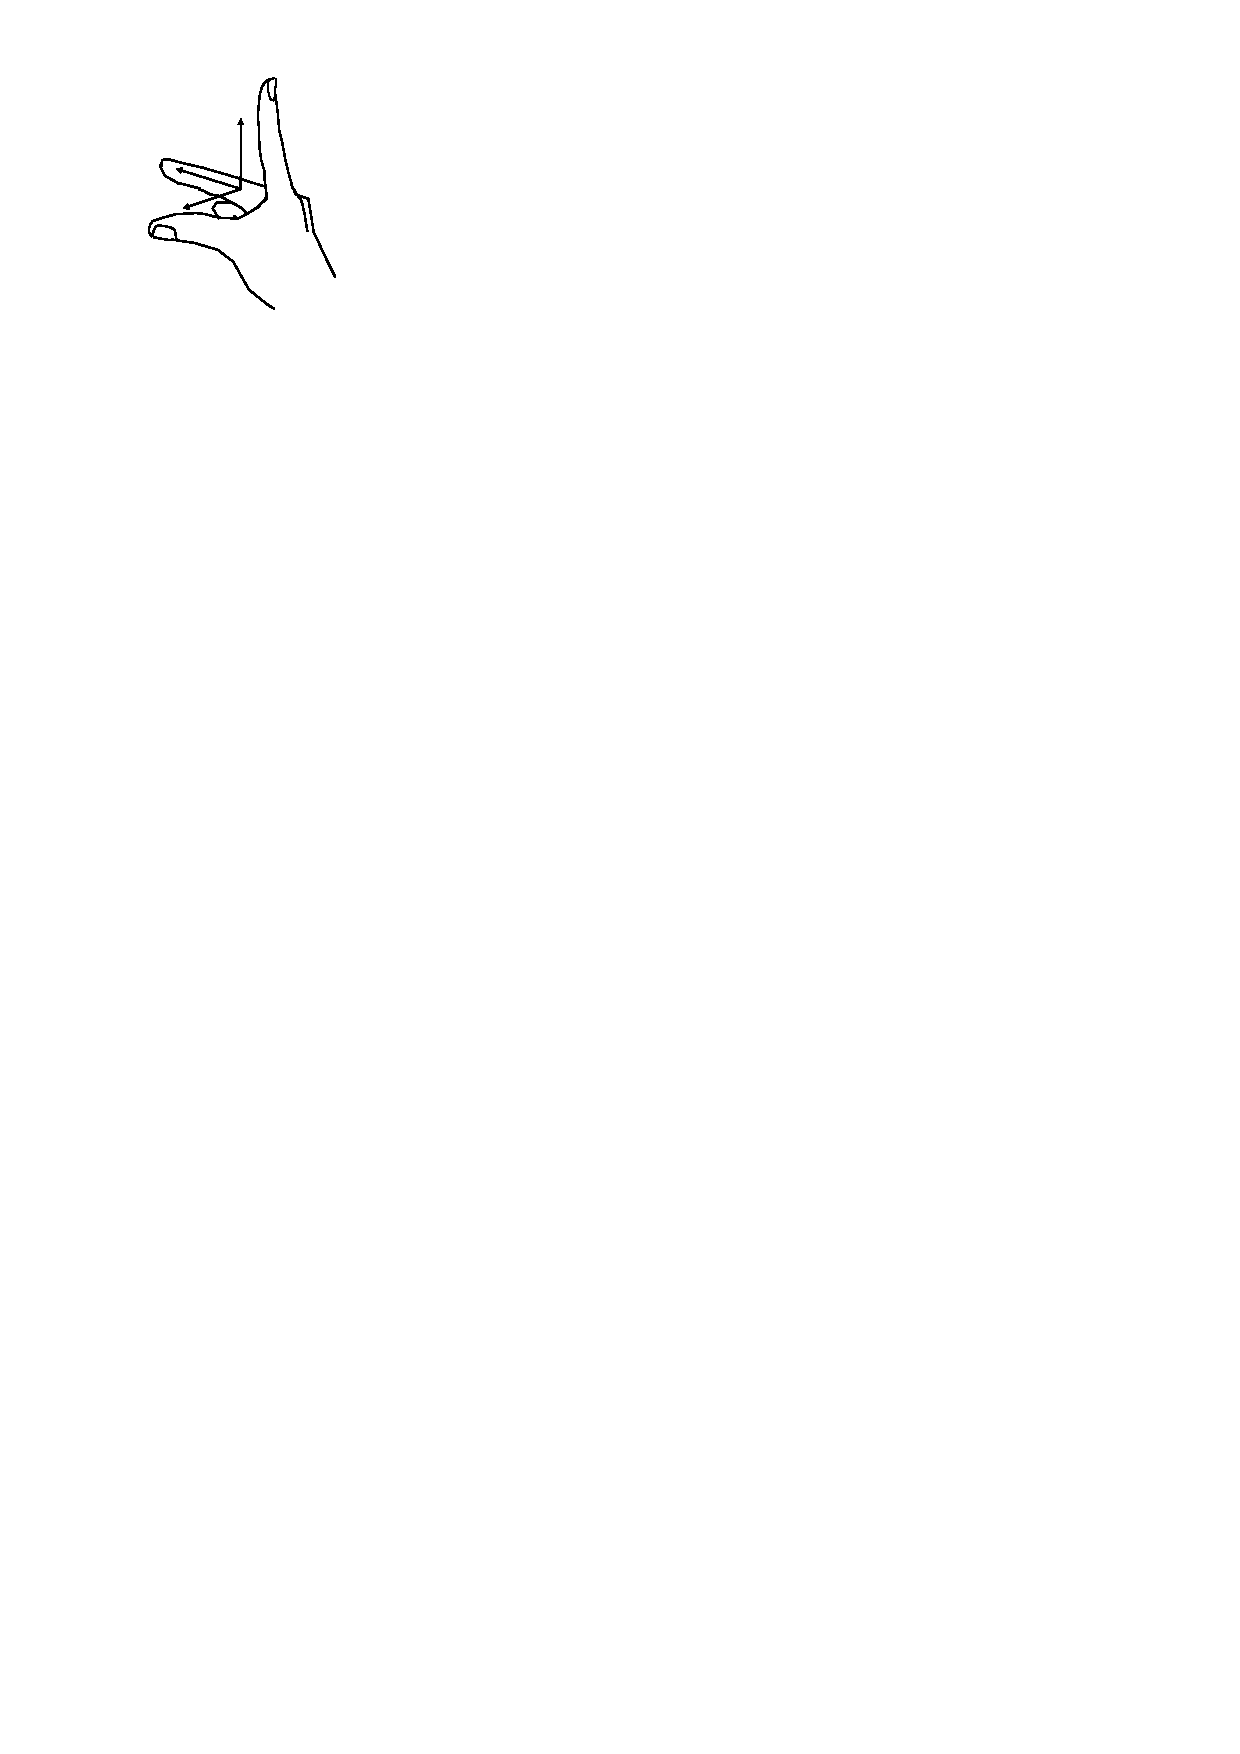
\includegraphics[width=3cm]{Src/Images/main}};
\draw (-1.1,-0.1) node {$\vx{}$};
\draw (-1.,0.7) node {$\vz{}$};
\draw (0,1.4) node {$\vy{}$};
\end{tikzpicture}
  \vspace{-2em}
\end{wrapfigure}
L'association de trois vecteurs indépendants forme une base \bB{} de $(E)$, noté  \base{\vx{}}{\vy{}}{\vz{}}. Tout vecteur $\vecteur{V}$ se décompose de manière unique sur cette base : \[\vecteur{V}=v_x.\vx{}+v_y.\vy{}+v_z.\vz{}\]

On utilisera en Sciences de l'Ingénieur des bases orthonormées directes $(\vx{}, \vy{}, \vz{})$,  c'est-à-dire des vecteurs orthogonaux, de même norme égale à 1. La base est directe si elle vérifie la \og règle de la main droite \fg{}.

\subsubsection{Repère}
Un repère est une base vectorielle associée à un point appelé origine. En mécanique du solide, on a l'habitude d'associer un repère \repere[\rR{i}]{O_i}{\vx{i}}{\vy{i}}{\vz{i}} à chaque solide $S_i$.

\UPSTIremarque{En Sciences de l'Ingénieur, les notions de bases et de repère sont appréciées de manières identiques.}

\subsubsection{Expression d'un vecteur dans différents repères}
Considérons un système de solides $S_1$ et $S_2$ liés par une articulation (pivot) de centre $A$ et d'axe perpendiculaire au plan de la feuille. Considérons le point $B$ appartenant au solide $S_2$ à une distance $L$ de $A$. Le solide $S_1$ est fixe par rapport à la feuille. À l'instant $t_1$ le système est en position 1, considérons le vecteur $\vecteur{AB_1}$, puis à l'instant $t_2$ le système est en position 2, considérons le vecteur $\vecteur{AB_2}$. Pour caractériser ces deux vecteurs nous pouvons les exprimer dans une base (un repère). Le choix de la base est arbitraire, soit \repere[\rR1]{A}{\vx1}{\vy1}{\vz1} base orthonormé définie sur la figure en position 1 ou \repere[\rR2]{A}{\vx2}{\vy2}{\vz2} base orthonormé définie sur la figure en position 2. 

\begin{figure}[!ht]
\centering
\begin{tikzpicture}[scale=1.1]
\begin{scope}
\draw (2,3) node {Position 1};
\draw[thick] (-1,-1) node[above right] {$S_1$} rectangle (2.5,0.2);
\draw[very thick,UPSTIcustomColor1] (2,0) node[below,yshift=-2mm,black] {$S_2$} ellipse (2.5 and 0.7);
\draw[->,>=latex] (0,0) node[left,xshift=1mm,yshift=-1mm] {$\vec z_1$} -- (3,0) node[above] {$\vx{}_1$};
\draw[->,>=latex] (0,0) -- (0,3) node[above] {$\vec y_1$};
\draw (4,0) node {$+$} node[below left] {$B_1$};
\draw (0,0) node {$\circ$} node[below right] {$A$};
\end{scope}
\begin{scope}[xshift=7cm]
\draw (2,3) node {Position 2};
\draw[thick] (-1,-1) node[above right] {$S_1$} rectangle (2.5,0.2);
\draw[dashed,UPSTIcustomColor1] (2,0) node[below,yshift=-2mm,black] {$S_2$} ellipse (2.5 and 0.7);
\draw[->,>=latex] (0,0) node[left,xshift=1mm,yshift=-1mm] {$\vec z_1$} -- (3,0) node[above,xshift=3mm,yshift=-1mm] {$\vx{}_1$};
\draw[->,>=latex] (0,0) -- (0,3) node[above] {$\vec y_1$};
\draw (4,0) node {$+$} node[below left] {$B_1$};
\draw (0,0) node {$\circ$} node[below right] {$A$};
\draw[->,>=latex] (2,0) arc(0:20:2) ;
\draw (10:2.2) node {$\alpha$};
\end{scope}
\begin{scope}[xshift=7cm,rotate=20]
\draw[very thick,UPSTIcustomColor1] (2,0) ellipse (2.5 and 0.7);
\draw[->,>=latex] (0,0) -- (3,0) node[above] {$\vx{}_2$};
\draw[->,>=latex] (0,0) -- (0,3) node[above] {$\vec y_2$};
\draw (4,0) node {$+$} node[below left] {$B_2$};
\end{scope}
\end{tikzpicture}
\end{figure}

\vspace{1em}
Notons $L$ la longueur du segment $[AB]$. Dans la position 1, on a $\vecteur{AB_1}=L.\vx1$ dans le repère \rR1.

Dans la position 2, on a $\vecteur{AB_2}=L.\vx2$ dans le repère \rR2. Mais aussi $\vecteur{AB_2}=L\cos\alpha.\vx1+L\sin\alpha.\vy1$ dans le repère \rR1.

\subsection{Produit scalaire}
\subsubsection{Définition}
\UPSTIdefinition[Produit scalaire]{
Le produit scalaire de deux vecteurs est un \textbf{nombre}, noté $\vu{} \cdot \vecteur{v}$  tel que:
\[\vu{} \cdot \vecteur{v} = \norme{\vu{}}\times\norme{\vecteur{v}}\times \cos(\vu{},\vecteur{v})\]
\vspace{-1em}
}

\noindent En SII, on manipule essentiellement des vecteurs unitaires. Dans ce cas, en admettant que $\couple{\vu{}}{\vecteur{v}}=\theta$:
\[\vu{} \cdot \vecteur{v}=\cos\theta\]

\subsubsection{Propriétés}
\begin{itemize}
\item Commutativité :  $\vu{} \cdot \vecteur{v} = \vecteur{v} \cdot \vu{}$;
\item Distributivité :  $\vu{} \cdot (\vecteur{v}+\vw{}) = \vu{} \cdot \vecteur{v}+ \vu{} \cdot \vw{}$;
\item Linéarité :  $\lambda.\vu{} \cdot \mu.\vecteur{v} = \lambda\mu\left(\vu{} \cdot \vecteur{v}\right)$;
\item Si $\vu{} \cdot \vecteur{v}=0$ alors $\vu{} = \vec 0$ ou $\vecteur{v}=\vec 0$ ou $\vu{} \perp \vecteur{v}$;
\item Si $\vu{} \sslash \vecteur{v}$ alors on a $\vu{} \cdot \vecteur{v}=\varepsilon \norme{\vu{}} \times \norme{\vecteur{v}}$ avec $\varepsilon = \pm 1$ suivant l'orientation de $\vu{}$  et $\vecteur{v}$.
\end{itemize}


\subsubsection{Expression analytique}
\begin{wrapfigure}{r}{6cm}
  \centering
  \vspace{-2em}
\begin{tikzpicture}
\coordinate (a) at (0,0);
\draw (a) -- ++(200:0.5);
\draw (a) -- ++(20:5.5);
\draw[very thick,|->,>=latex,UPSTIcustomColor1] (a) -- ++(20:1) node[midway,above left,black] {$\vu{}$} ;
\draw[very thick,->,>=latex,UPSTIcustomColor1] (a)++(20:2) node[inner sep =0] (b) {} -- ++(20:3) node [midway, above,black] {$\vecteur{p}$} node[inner sep=0] (c) {};
\draw (b) -- ++(110:0.5);
\draw (c) -- ++(110:1.5) node[inner sep=0,outer sep=0] (c1) {};
\draw[very thick,->,>=latex,UPSTIcustomColor1] (b)++(110:0.5) -- (c1) node[midway,above left,black] {$\vecteur{V}$};
\draw (b)++(110:0.3) -- ++(20:0.3) -- ++(-70:0.3);
\draw (c)++(110:0.3) -- ++(20:0.3) -- ++(-70:0.3);
\end{tikzpicture}
  \vspace{-3em}
\end{wrapfigure}

Dans une base orthonormée \bxyz, on peut montrer que le produit scalaire entre $\vu{}$ et $\vecteur{v}$ est défini par la relation entre les coordonnées :  \[\vu{} \cdot \vecteur{v} = u_x v_x+u_y v_y+ u_z v_z\]

\subsubsection{Interprétation géométrique}
Soit $\vecteur{p}$  la projection vectorielle d'un vecteur $\vecteur{V}$ sur une droite de vecteur directeur $\vu{}$ ( unitaire ) alors:  \[\vecteur{p} = (\vecteur{V} \cdot \vu{}).\vu{}\]


\subsection{Changement de bases}
\subsubsection{Principe}

Dans la pratique, la lecture de figure spatiale étant délicate, on se ramène toujours à des figures planes. Dans la plupart des cas, le passage d'une base à une autre est réalisé par \textbf{une rotation plane}.

\begin{wrapfigure}{r}{5cm}
  \centering
  \setCouleursParametrage{black}{UPSTIcustomColor1}  
  \parametrageAngulaire{\theta}{\vx1}{\vy1}{\vz1}{\vx2}{\vy2}[\vz2]
	\vspace{-6em} 
\end{wrapfigure}
Pour faciliter le calcul des projections, on utilise des figures géométrales appelées aussi figures de projection ou figures de calcul ou figures de changement de bases. 

\UPSTIattention{Ces figures seront toujours réalisées avec des angles positifs proche de 20°, le vecteur commun aux deux bases étant perpendiculaire à la feuille toujours dirigé vers le lecteur de la figure.}

Vous devez être capables de retrouver les projections des différents vecteurs \textbf{sans hésitation}:
\[\begin{array}{r@{\,=\,}l@{\qquad\qquad\qquad} r@{\,=\,}l}
\vx2 & \cos\theta.\vx1 +\sin\theta.\vy1 &
\vy2 & \cos\theta.\vy1 -\sin\theta.\vx1 \\
\vx1 & \cos\theta.\vx2 -\sin\theta.\vy2 &
\vy1 & \cos\theta.\vy2 +\sin\theta.\vx2
\end{array}\]

Pour éviter toute erreur, il est utile de vérifier ses formules de projection en $\theta$ = 0 et $\theta$ = \SI{90}{\degree}.

\subsubsection{Astuce de calcul avec les figures planes}
Quand on cherche à projeter un vecteur dans une autre base avec une figure plane, si on a bien dessiné la figure \textbf{avec un angle de 20° environ}, on voit apparaitre un triangle rectangle de la forme ci-dessous, avec un \og petit côté\fg{} et un \og grand côté\fg{}. Comme on raisonne sur des vecteurs unitaires, l'hypoténuse est de longueur égale à 1.

	\begin{center}
	\begin{tikzpicture}
    	\tikzstyle{flecheFigure}=[->, >=latex]
		\draw [flecheFigure, gray] (0,0) -- (2.2,0) node[right] {\vx1} ;
		\draw [flecheFigure, gray] (0,0) -- (0,2.2) node[above] {\vy1};
		\draw [anchor=north east] (-0.1,0) node {\textcolor{gray}{\vz1}\textcolor{black}{${\,=\vz2}$}};		

		\draw[UPSTIcustomColor1, very thick] (0,0) -- (2.1*0.9063,0);
		\draw[UPSTIcustomColor3, very thick] (2.1*0.9063,0) --++ (0,2.1*0.4226);
		\draw[UPSTIcustomColor4, very thick] (0,0) -- (0,2.1*0.9063);
		\draw[UPSTIcustomColor5, very thick] (0,2.1*0.9063) --++ (-2.1*0.4226,0);
		\begin{scope} [rotate=25]
			\draw [anchor=south west] (2,0) node {\textcolor{black}{\vx2}};
			\draw[->, >=latex, black, very thick] (0,0) -- (2.1,0);
			\draw[->, >=latex, black, very thick] (0,0) -- (0,2.1)node[above] {\textcolor{black}{\vy2}};
		\end{scope}
		
		\draw [flecheFigure, >=latex, color=gray](1,0) arc (0:25:1);
		\draw [anchor=center]({25/2}:1.25) node {\textcolor{gray}{$\theta$}};
		\draw[flecheFigure,rotate=90, color=gray] (1,0) arc (0:25:1);
		\draw [rotate=90,anchor=center]({25/2}:1.25) node {\textcolor{gray}{$\theta$}};
	    \fill[white] (0,0) circle (0.13);
	    \draw [flecheFigure,very thick] (0,0) circle (0.13);
	    \fill[black] (0,0) circle (0.03);
	    \draw [flecheFigure,thick] (0,0) circle (0.04);

		\begin{scope}[scale=2.5,xshift=1.9cm,yshift=0.25cm]
			
		\draw [flecheFigure, >=latex, color=gray](0.4,0) arc (0:25:0.4);
		\draw [anchor=center]({25/2}:0.5) node {\textcolor{gray}{$\theta$}};
			\draw[->, >=latex, very thick] (0,0) -- (25:1) node[midway, above] {$1$};
			\draw[UPSTIcustomColor1, very thick] (0,0) -- (0.9063,0) node[midway, below] {$\cos\theta$};
			\draw[UPSTIcustomColor3, very thick] (0.9063,0) --++ (0,0.4226) node[midway, right] {$\sin\theta$};

			\node at (0.5,-0.65) {$\vx2=\textcolor{UPSTIcustomColor1}{\cos\theta}.\vx1+\textcolor{UPSTIcustomColor3}{\sin\theta}.\vy1 $};

		\end{scope}
						
		\begin{scope}[scale=2.5,xshift=4.6cm,yshift=0.1cm]
		\begin{scope}[rotate=90]
		\draw [flecheFigure, >=latex, color=gray](0.4,0) arc (0:25:0.4);
		\draw [anchor=center]({25/2}:0.5) node {\textcolor{gray}{$\theta$}};
			\draw[->, >=latex, very thick] (0,0) -- (25:1) node[midway, left] {$1$};
			\draw[UPSTIcustomColor4, very thick] (0,0) -- (0.9063,0) node[midway, right] {$\cos\theta$};
			\draw[UPSTIcustomColor5, very thick] (0.9063,0) --++ (0,0.4226) node[midway, above] {$\sin\theta$};
	
		\end{scope}

			\node at (-0.1,-0.5) {$\vy2=\textcolor{UPSTIcustomColor5}{-\sin\theta}.\vx1+\textcolor{UPSTIcustomColor4}{\cos\theta}.\vy1 $};
		\end{scope}

	\end{tikzpicture}
	\end{center}
	
Il suffit alors de retenir que \textbf{\og petit côté\fg{} = sinus} et \textbf{\og grand côté\fg{} = cosinus}, et de raisonner sur la direction des vecteurs pour déduire le signe...

\subsection{Produit vectoriel}
\subsubsection{Définition}
\UPSTIdefinition[Produit vectoriel]{
Le produit vectoriel de deux vecteurs est un \textbf{vecteur}, noté $\vu{} \vect \vecteur{v}$  tel que:
\[\vu{} \vect \vecteur{v} = \norme{\vu{}}\times\norme{\vecteur{v}}\times \sin(\vu{},\vecteur{v}).\vw{} \]

\vspace{-0.5em}
\noindent avec \vw{} tel que \triplet{\vu{}}{\vecteur{v}}{\vw{}} forme un trièdre direct.
}

\noindent En SII, on manipule essentiellement des vecteurs unitaires. Dans ce cas, en admettant que $\couple{\vu{}}{\vecteur{v}}=\theta$:
\[\vu{} \vect \vecteur{v}=\sin\theta.\vw{}\]


\subsubsection{Propriétés}
\begin{itemize}
\item Distributivité :  $\vu{} \vect (\vecteur{v}+\vw{}) = \vu{} \vect \vecteur{v}+ \vu{} \vect \vw{}$;
\item Linéarité :  $\lambda.\vu{} \vect \mu.\vecteur{v} = \lambda\mu\left(\vu{} \vect \vecteur{v}\right)$;
\item Anti-symétrie :  $\vu{} \vect \vecteur{v} = -\vecteur{v} \vect \vu{}$.
\end{itemize}

\subsubsection{Astuce de calcul}
Lorsque les 2 termes du produit vectoriel sont 2 vecteurs d'une base  orthonormée directe (exemple: $\vx{}\vect\vy{}$), on peut facilement calculer le produit vectoriel en utilisant le moyen mnémotechnique suivant:


\begin{center}
\begin{tikzpicture}
\node at (0,0) {\huge $x\quad y\quad z\quad x\quad y\quad z$};

\begin{scope}[shift={(-1.7,0.4)}]
	\draw[<-, >=latex, UPSTIcustomColor1] (0,0) arc (25:150:0.5) node[midway, above] {$\oplus$};
\end{scope}
\begin{scope}[shift={(-0.6,0.4)}]
	\draw[<-, >=latex, UPSTIcustomColor1] (0,0) arc (25:150:0.5) node[midway, above] {$\oplus$};
\end{scope}
\begin{scope}[shift={(0.5,0.4)}]
	\draw[<-, >=latex, UPSTIcustomColor1] (0,0) arc (25:150:0.5) node[midway, above] {$\oplus$};
\end{scope}

\begin{scope}[yscale=-1]
\begin{scope}[shift={(-1.7,0.4)}]
	\draw[->, >=latex, UPSTIcustomColor3] (0,0) arc (30:155:0.5) node[midway, below] {$\ominus$};
\end{scope}
\begin{scope}[shift={(-0.6,0.4)}]
	\draw[->, >=latex, UPSTIcustomColor3] (0,0) arc (30:155:0.5) node[midway, below] {$\ominus$};
\end{scope}
\begin{scope}[shift={(0.5,0.4)}]
	\draw[->, >=latex, UPSTIcustomColor3] (0,0) arc (30:155:0.5) node[midway, below] {$\ominus$};
\end{scope}
\end{scope}

\end{tikzpicture}
\end{center}


\subsubsection{Encore une astuce, en utilisant les figures planes}
Lorsque les 2 termes ne font pas partie de la même base (exemple: $\vx1\vect\vx0$), on peut éviter de projeter \vx1 dans la base \bB0 en utilisant la méthode suivante, dite \og méthode à 3 temps\fg{}, expliquée sur les 2 exemples suivants:

\vspace{-1em}
\begin{center}
  \setCouleursParametrage{black}{UPSTIcustomColor1}  
  \parametrageAngulaire{\theta}{\vx1}{\vy1}{\vz1}{\vx2}{\vy2}[\vz2]

\end{center}

\noindent
\begin{minipage}[t]{0.45\linewidth}
\begin{center}
\Large
$\vy1\vect\vy2=?$
\end{center}

\vspace{0.5em}
\begin{enumerate}
\item Pour aller de $\vy1$ vers $\vy2$, on \og tourne\fg{} autour de $\textcolor{UPSTIcustomColor1}{\vz1}$;
\item On \og tourne\fg{} dans le sens \textcolor{UPSTIcustomColor4}{positif};
\item L'angle entre les 2 est $\textcolor{UPSTIcustomColor3}{\theta}$.
\end{enumerate}

\vspace{0.5em}
\begin{center}
$\UPSTIcadreMath{\vy1\vect\vy2=\textcolor{UPSTIcustomColor4}{+}\sin\textcolor{UPSTIcustomColor3}{\theta}.\textcolor{UPSTIcustomColor1}{\vz1}}$
\end{center}
\end{minipage} \hfill
\begin{minipage}[t]{.45\linewidth}
\begin{center}
\Large
$\vy2\vect\vx1=?$
\end{center}

\vspace{0.5em}
\begin{enumerate}
\item Pour aller de $\vy2$ vers $\vx1$, on \og tourne\fg{} autour de $\textcolor{UPSTIcustomColor1}{\vz1}$;
\item On \og tourne\fg{} dans le sens \textcolor{UPSTIcustomColor4}{négatif};
\item L'angle entre les 2 est $\textcolor{UPSTIcustomColor3}{\frac{\pi}{2}+\theta}$.
\end{enumerate}

\vspace{0.5em}
\begin{center}
$\UPSTIcadreMath{\vy2\vect\vx2=\textcolor{UPSTIcustomColor4}{-}\sin\left(\textcolor{UPSTIcustomColor3}{\frac{\pi}{2}+\theta}\right).\textcolor{UPSTIcustomColor1}{\vz1}=\textcolor{UPSTIcustomColor4}{-}\textcolor{UPSTIcustomColor3}{\cos\theta}.\textcolor{UPSTIcustomColor1}{\vz1}}$
\end{center}
\end{minipage} 


\vspace{1em}
\UPSTIattention{On ne peut utiliser cette méthode que s'il existe une figure plane sur laquelle apparaissent les 2 termes du produit vectoriel. Dans le cas contraire, on n'échappera pas à des calculs de projection.}

\subsection{Produit mixte}
\UPSTIdefinition[Produit mixte]{
Le produit mixte est la quantité notée \triplet{\vu{}}{\vecteur{v}}{\vw{}} et définie par:
\[\triplet{\vu{}}{\vecteur{v}}{\vw{}}=\prodMixte{\vu{}}{\vecteur{v}}{\vw{}} \]
\vspace{-1em}
}


Le produit mixte se conserve par permutation circulaire:
\[ \triplet{\vu{}}{\vecteur{v}}{\vw{}} = \triplet{\vecteur{v}}{\vw{}}{\vu{}} = \triplet{\vw{}}{\vu{}}{\vecteur{v}} \Longleftrightarrow \prodMixte{\vu{}}{\vecteur{v}}{\vw{}} = \prodMixte{\vecteur{v}}{\vw{}}{\vu{}} = \prodMixte{\vw{}}{\vu{}}{\vecteur{v}}\]

Utiliser les propriétés du produit mixte permet parfois de simplifier spectaculairement les calculs (de dynamique, notamment...).


\subsection{Dérivation vectorielle}
\subsubsection{Dérivation directe}
Soit un vecteur \vecteur{V} repéré dans \rROxyz{} par $\vecteur{V}=x.\vx{}+y.\vy{}+z.\vz{}$. La dérivée temporelle de ce vecteur par rapport au repère \rR{} s'écrit:
\[ \derivV{\vecteur{V}}{\rR{}}=\deriv{x}.\vx{}+x.\derivV{\vx{}}{\rR{}}+\deriv{y}.\vy{}+y.\derivV{\vy{}}{\rR{}}+\deriv{z}.\vz{}+z.\derivV{\vz{}}{\rR{}} \]

Les vecteurs \vx{}, \vy{} et \vz{} étant fixes (ie constants au cours du temps) dans le repère \rR{}, leurs dérivées sont nulles, donc: 
\[ \derivV{\vecteur{V}}{\rR{}}=\deriv{x}.\vx{}+\deriv{y}.\vy{}+\deriv{z}.\vz{} \]

Pour simplifier les écritures, en SII on note souvent $\deriv{u}=\dot{u}$, d'où:
\[ \derivV{\vecteur{V}}{\rR{}}=\xp.\vx{}+\yp.\vy{}+\zp.\vz{} \]

\subsubsection{Dérivation composée}
Très souvent en SII, les expressions vectorielles ne sont pas exprimées dans un unique repère (exemple: $\vecteur{V}=a.\vy2+b.\vz1+c.\vx0$). La dérivation vectorielle n'est plus aussi aisée. 

Les étudiants sont souvent tentés de tout projeter dans \rR0 avant de dériver, ce qui est une bien mauvaise idée (souvent héritée de la mécanique du point vue en Physique).

En SII, on privilégiera donc l'utilisation de la formule de dérivation vectorielle (dite \og formule de Bour\fg{}):

\UPSTIdefinition[Formule de Bour]{
\[ \Bour{\vu{}}{\rR1}{\rR0} \]
}

\subsubsection{Astuce de calcul avec les figures planes}
Si on cherche à dériver un vecteur \vu{i} dans un repère \rR{j}, et qu'il existe \textbf{une même figure plane} sur laquelle \vu{i} et \rR{j} apparaissent, alors on peut utiliser la méthode suivante: si on considère la figure plane ci-dessous à gauche, et qu'on souhaite calculer \derivV{\vx2}{\rR1}, il faut:
\begin{itemize}
\item faire faire une rotation de $-\frac{\pi}{2}$ au vecteur \vx2, ce qui nous donne \vy2;
\item multiplier ce vecteur par la dérivée temporelle de l'angle défini sur la figure plane: $\thetap$.
\end{itemize}

On trouve alors:\quad $\UPSTIcadreMath{\derivV{\vx2}{\rR1}=\thetap.\vy2}$

Par la même méthode, la figure  ci-dessous à droite donne immédiatement:\quad $\UPSTIcadreMath{\derivV{\vy2}{\rR1}=-\thetap.\vx2}$

\noindent
\begin{minipage}[c]{0.45\linewidth}
	\centering
  \setCouleursParametrage{black}{UPSTIcustomColor1}  
  \parametrageAngulaire{\theta}{\vx1}{\vy1}{\vz1}{\vx2}{\vy2}[\vz2]
\end{minipage} \hfill
\begin{minipage}[c]{.45\linewidth}
	\centering

\begin{tikzpicture}
   \tikzstyle{flecheFigure}=[->, >=latex]
	\draw [flecheFigure,very thick] (0,0) -- (1.8,0) ;
	\draw [flecheFigure,very thick] (0,0) -- (0,1.8) ;
	\draw [anchor=north west] (1.7,0) node {\vx1};
	\draw [anchor=south west] (0,1.7) node {\vy1};

	\begin{scope} [rotate=25]
		\draw [flecheFigure, color=UPSTIcustomColor1] (0,0) -- (1.8,0) ;
		\draw [flecheFigure, color=UPSTIcustomColor1] (0,0) -- (0,1.8) ;
		\draw [flecheFigure, color=UPSTIcustomColor1, dashed] (0,0) -- (-1.8,0) ;
		\draw [anchor=south west] (1.7,0) node {\textcolor{UPSTIcustomColor1}{\vx2}};
		\draw [anchor=north east] (0,1.8) node {\textcolor{UPSTIcustomColor1}{\vy2}};
		\draw [anchor=south east] (-1.7,0) node {\textcolor{UPSTIcustomColor1}{-\vx2}};
		
		\draw[flecheFigure, UPSTIcustomColor3, very thick] (15:2.5) arc (15:80:2.5) node[midway, above] {$+\dfrac{\pi}{2}$};

		\draw[flecheFigure, UPSTIcustomColor3, very thick] (105:2.5) arc (105:170:2.5) node[midway, left] {$+\dfrac{\pi}{2}$};
	\end{scope}
	
	\draw [flecheFigure, >=latex, color=UPSTIcustomColor1](1,0) arc (0:25:1);
	\draw [anchor=center]({25/2}:1.25) node {\textcolor{UPSTIcustomColor1}{$\theta$}};
	\draw[flecheFigure,rotate=90, color=UPSTIcustomColor1] (1,0) arc (0:25:1);
	\draw [rotate=90,anchor=center]({25/2}:1.25) node {\textcolor{UPSTIcustomColor1}{$\theta$}};
	
\end{tikzpicture}


\end{minipage} 

\vspace{1em}
\UPSTIattention{On ne peut utiliser cette méthode que s'il existe une figure plane sur laquelle apparaissent le vecteur à dériver \textbf{et} le repère (ou base) dans lequel on souhaite dériver. Dans le cas contraire, on n'échappera pas là encore à des calculs de projection.}




\end{document}
